\subsection{积分理论}

定义 13. --- 设 \(p \in [1, +\infty[\) ；用 \(\overline{\mathcal{L}}^p(T, \mu)\) （相应地 \(\overline{\mathcal{L}}_F^p(T, \mu)\) ，若 \(F\) 是 Banach 空间）表示映射 \(f\) （从 \(T\) 到 \(\overline{R}\) ，相应地到 \(F\) ）中 \(\mu\) -可测且满足 \(\mu^\bullet(|f|^p) < +\infty\) 者的全体。用 \(\mathcal{L}^p(T, \mu)\) （相应地 \(\mathcal{L}_F^p(T, \mu)\) ）表示 \(\mu\) -适度元素（\(\overline{\mathcal{L}}^p(T, \mu)\) 中的，相应地 \(\overline{\mathcal{L}}_F^p(T, \mu)\) 中的）全体。

我们记 \(\overline{\mathbf{N}}_p(\mathbf{f}) = (\mu^\bullet (|\mathbf{f}|^p))^{1 / p}\) ，\(\mathrm{N}_p(\mathbf{f}) = (\mu^* (|\mathbf{f}|^p))^{1 / p}\) 。用 \(\overline{\mathrm{N}}_{\infty}(\mathbf{f})\) 表示数 \(k\geqslant 0\) （使 \(|\mathbf{f}|\leqslant k\) 局部 \(\mu\) -几乎处处成立）的下确界；若 \(\overline{\mathrm{N}}_{\infty}(\mathbf{f}) < + \infty\) ，则称 \(\mathbf{f}\) 本性有界。T 到 \(\overline{\mathbf{R}}\) （相应地到 F）中的可测且本性有界的映射全体记作 \(\overline{\mathcal{L}}^{\infty}(\mathrm{T},\mu)\) （相应地 \(\overline{\mathcal{L}}_{\mathrm{F}}^{\infty}(\mathrm{T},\mu)\) ）。\(\overline{\mathcal{L}}_{\mathrm{F}}^{1}(\mathrm{T},\mu)\) （相应地 \(\mathcal{L}_{\mathrm{F}}^{1}(\mathrm{T},\mu)\)）的元素称为以 F 为值的本性可积函数（相应地可积函数）。

若 \(\mu\) 是复测度，则令

\[
\overline {{{{\mathcal {L}}}}} _ {\mathrm{F}} ^ {p} (\mathrm{T}, \mu) = \overline {{{{\mathcal {L}}}}} _ {\mathrm{F}} ^ {p} (\mathrm{T}, | \mu |) \quad \text { and } \quad \mathcal {L} _ {\mathrm{F}} ^ {p} (\mathrm{T}, \mu) = \mathcal {L} _ {\mathrm{F}} ^ {p} (\mathrm{T}, | \mu |).
\]

只要不引起混淆，上述记号常缩写为 \(\overline{\mathcal{L}}_F^p (\mu)\) 、\(\overline{\mathcal{L}}_F^p\) 或 \(\mathcal{L}^p (\mu)\) 、\(\mathcal{L}^p\) 。

我们在 No.~8（附论）中看到，可以构造一个局部紧空间 \(\mathbf{T}'\) ，它与 \(\mathbf{T}\) 有同一底层集合且拓扑比 \(\mathbf{T}\) 更细，并在 \(\mathbf{T}'\) 上配备测度 \(\mu'\) ，使 \(\mu\) -可测函数与 \(\mu'\) -可测函数相同，且正函数对 \(\mu\) 与 \(\mu'\) 的本质上积分相等。由此推出，集合 \(\overline{\mathcal{L}}_{\mathrm{F}}^{p}(\mu)\) 与 \(\overline{\mathcal{L}}_{\mathrm{F}}^{p}(\mu')\) 对 \(1 \leqslant p \leqslant +\infty\) 相同。(1) 这也使我们无需新证明即可断言 \(\overline{\mathcal{L}}_{\mathrm{F}}^{p}\) 是向量空间，函数 \(\overline{\mathrm{N}}_p\) 是 \(\overline{\mathcal{L}}_{\mathrm{F}}^{p}(\mu)\) 上的半范数，且该空间对此完备。

设 \(\mathbf{f}\) 是 \(\overline{\mathcal{L}}_{\mathrm{F}}^{p}\) 的元素 ( \(1 \leqslant p < +\infty\) )；由于 \(\mu^{\bullet}(|\mathbf{f}|^{p}) = \mu^{\prime \bullet}(|\mathbf{f}|^{p}) < +\infty\) ，Ch. V, §1, No.~2 的 Prop. 7 蕴含 \(\mathbf{f}\) 在 \(\mathbf{T}'\) 的一列紧子集与一个局部 \(\mu'\) -可忽略集之并外为零；后一集局部 \(\mu\) -可忽略，且 \(\mathbf{T}'\) 的每个紧子集在 \(\mathbf{T}\) 中紧，由此 \(\mathbf{f}\) 局部 \(\mu\) -几乎处处等于一个 \(\mu\) -适度函数。用 \(\overline{\mathcal{N}}_{\mathrm{F}}\) （相应地 \(\mathcal{N}_{\mathrm{F}}\) ）表示局部 \(\mu\) -可忽略（相应地 \(\mu\) -可忽略）函数空间；于是有 \(\overline{\mathcal{L}}_{\mathrm{F}}^{p} = \mathcal{L}_{\mathrm{F}}^{p} + \overline{\mathcal{N}}_{\mathrm{F}}\) ，且 \(\mathcal{N}_{\mathrm{F}} = \mathcal{L}_{\mathrm{F}}^{p} \cap \overline{\mathcal{N}}_{\mathrm{F}}\) (No.~9, Prop. 14 的 Cor. 1)。因此空间 \(\overline{\mathcal{L}}_{\mathrm{F}}^{p} / \overline{\mathcal{N}}_{\mathrm{F}}\) 可以典范地等同于 \(\mathcal{L}_{\mathrm{F}}^{p} / \mathcal{N}_{\mathrm{F}}\) ，且立即可以验证这一等同保持范数；此商空间记作 \(\mathrm{L}_{\mathrm{F}}^{p}(\mu)\) 。它可以解释为与两个半范数空间 \(\overline{\mathcal{L}}_{\mathrm{F}}^{p}(\mu)\) 与 \(\mathcal{L}_{\mathrm{F}}^{p}(\mu)\) 中每一个相联系的赋范空间；由于 \(\overline{\mathcal{L}}_{\mathrm{F}}^{p}\) 完备，\(\mathrm{L}_{\mathrm{F}}^{p}\) 与 \(\mathcal{L}_{\mathrm{F}}^{p}\) 亦然。

函数 \(\mathbf{f}\) （以 \(\mathbf{F}\) 为值、在 \(\mathbf{T}'\) 上连续且具紧支集）全体在 \(\overline{\mathcal{L}}_{\mathbf{F}}^{p}(\mu') = \overline{\mathcal{L}}_{\mathbf{F}}^{p}(\mu)\) 中稠密 (Ch. IV, §3, No.~4, Def. 2)。重新采用 No.~8 的附论中的记号。由于 \(\mathbf{T}'\) 的紧子集只与有限个紧集 \(\mathbf{K}_{\alpha}\) 相交，每个具紧支集的连续函数 \(\mathbf{f}\) （在 \(\mathbf{T}'\) 上）都可写成和

\[
\mathbf {f} = \sum_ {\alpha \in A} \mathbf {f} _ {\alpha} + \mathbf {g},
\]

其中 \(f_{\alpha}\) 对每个 \(\alpha\) 是 \(K_{\alpha}\) 上一个连续函数经 0 延拓得到的函数，除有限个指标外 \(f_{\alpha}=0\) ，而 g 局部 \(\mu\) -可忽略。于是得到下列结果：

命题 15. --- 以 F 为值、使 Supp(f) 紧且 f 到 Supp(f) 的限制连续的函数 f 全体，在 \(\overline{\mathcal{L}}_{\mathrm{F}}^{p}(\mu)\) 与 \(\mathcal{L}_{\mathrm{F}}^{p}(\mu)\) 中稠密，其中 \(1 \leqslant p < +\infty\) 。

\pandocbounded{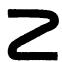
\includegraphics[keepaspectratio]{images/part002_287b28a9.jpg}}

注意这些函数并不是 T 上具紧支集的连续函数。

现在转到积分的定义。

命题 16. --- 存在且只存在一个连续线性映射 \(\mathbf{f} \mapsto \int \mathbf{f} d\mu\) ，它把空间 \(\overline{\mathcal{L}}_{\mathrm{F}}^{1}(\mu)\) 映到 \(\mathrm{F}\) 中，具有下列性质：

若 \(\mathbf{f}\) 形如 \(t \mapsto g(t)\mathbf{a}\) ，其中 \(\mathbf{a} \in \mathbf{F}\) ，\(g\) 是有限、\(\mu\) -可测的正函数且 \(\mu^{\bullet}(g) < +\infty\) ，则 \(\int \mathbf{f} d\mu = \mu^{\bullet}(g) \cdot \mathbf{a}\) 。

因为半范数空间 \(\overline{\mathcal{L}}_{\mathrm{F}}^{1}(\mu)\) 与 \(\overline{\mathcal{L}}_{\mathrm{F}}^{1}(\mu')\) 相同。由于 \(\mu^{\bullet} = \mu'^{\bullet}\) ，映射 \(\mathbf{f} \mapsto \int \mathbf{f} d\mu'\) 满足陈述中的条件。另一方面，陈述中所考虑的形如 \(\mathbf{f} = g \cdot \mathbf{a}\) 的函数全体在 \(\overline{\mathcal{L}}_{\mathrm{F}}^{1}(\mu')\) 中完全 (Ch. IV, §3, No.~5, Prop. 10)，由此得唯一性。

称 \(\int f d\mu\) 为 f 关于 \(\mu\) 的积分，这个向量也记作 \(\mu(\mathbf{f})\) 或 \(\int \mathbf{f}(t) d\mu(t)\) 。

由于对每个以 F 为值的本性可积函数 f 有 \(\int f d\mu = \int f d\mu'\) ，本质积分的全部理论无需新证明即可推广到 Hausdorff 空间上的测度；由它出发，把自身限制于适度函数，便得到关于通常积分的结果。我们特别引用下列结果：

--- Ch. IV, §3, No.~4 的 Th. 3，它到 \(\overline{\mathcal{L}}_{\mathrm{F}}^{p}\) 的推广，以及它的两个推论。

--- Ch. IV, §3, No.~5 的 Th. 4（与连续线性映射的复合）及其推论；同一 No. 的 Props. 9、11 与 12。

--- Ch. IV, §3, No.~6 中关于 \(L^{p}\) 的序向量空间结构的全部结果。

--- Ch. IV, §3, No.~7 的全部结果，特别是 Lebesgue 定理。

--- Ch. IV, §3, No.~8 中关于空间 \(L_F^p\) 之间关系的全部结果。

--- Ch. IV, §4, No.~3 的 Theorem 2（Lebesgue 定理对 \(L_F^1\) 的特殊陈述）。

--- Hölder 不等式 (Ch. IV, §6, No.~4, Th. 2) 及其推论。

--- Ch. IV, §6, No.~5 中建立的空间 \(L_{F}^{p}\) 之间的关系。

-- Ch. V, §5, No.~8 中建立的空间 \(\mathbf{L}^p\) 的对偶性结果。

--- Dunford--Pettis 定理 (Ch. VI, §2, No.~5, Th. 1)、其 Corollaries 1 与 2，以及 Ch. VI, §2, No.~6 的 Prop. 10（\(L_{F}^{1}\) 的对偶）。

